\chapter{Results}
% This should be 3000 words split with the methods
This section of the thesis will follow a chronological format  with some discussion of the conducted data analysis intermixed. This is as the validation results lead into each other, step by step.

\section{Response Times \& Task Construction Verification}
As the primary package of work within this project, verification of the task's ability to perform its intended acts is a critical result. The first step in any examination of any DN task is to examine the response time of the subjects to the stimuli in question. These were gathered from the behavioural data by finding when a stimulus was visible and recording the first key stroke. If the first key stroke was below a reasonable minimum human reaction time, taken to be 200ms it was discarded \citep{jainComparativeStudyVisual2015}. The next step was to desegregate that data between both stimulus options and both available choices. These plots can be seen below in figure \ref{fig:RT_B} \& \ref{fig:RT_C}


% Response Time Plots
\begin{figure}[H]
    \centering
    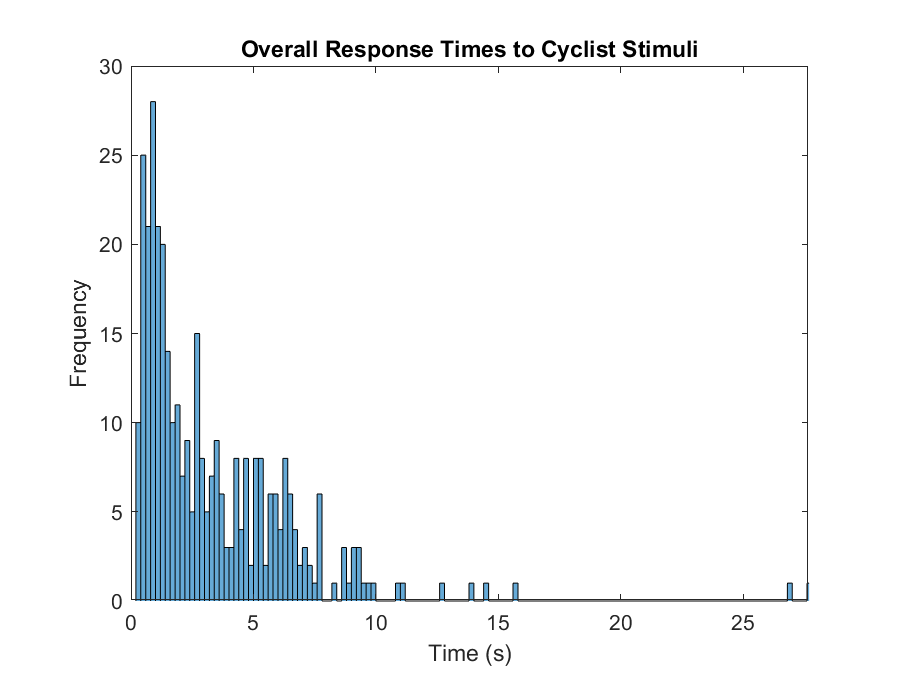
\includegraphics[width=0.37\paperwidth]{figures/BikeReactionTimes.eps}
    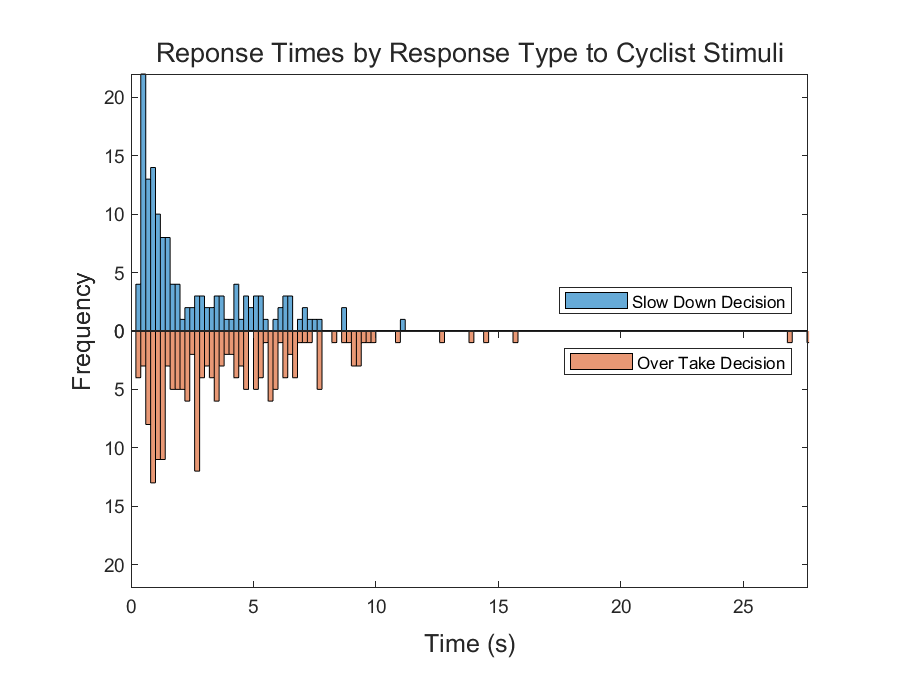
\includegraphics[width=0.37\paperwidth]{figures/BikeReactionTimes2.eps}
    \caption{Non-Subject Specific Distribution of Response Times to the 'Cyclist' Stimulus. a) Not Segregated by Response Type b) Segregated by Response Type}
    \label{fig:RT_B}
\end{figure}
\begin{figure}[H]
    \centering
    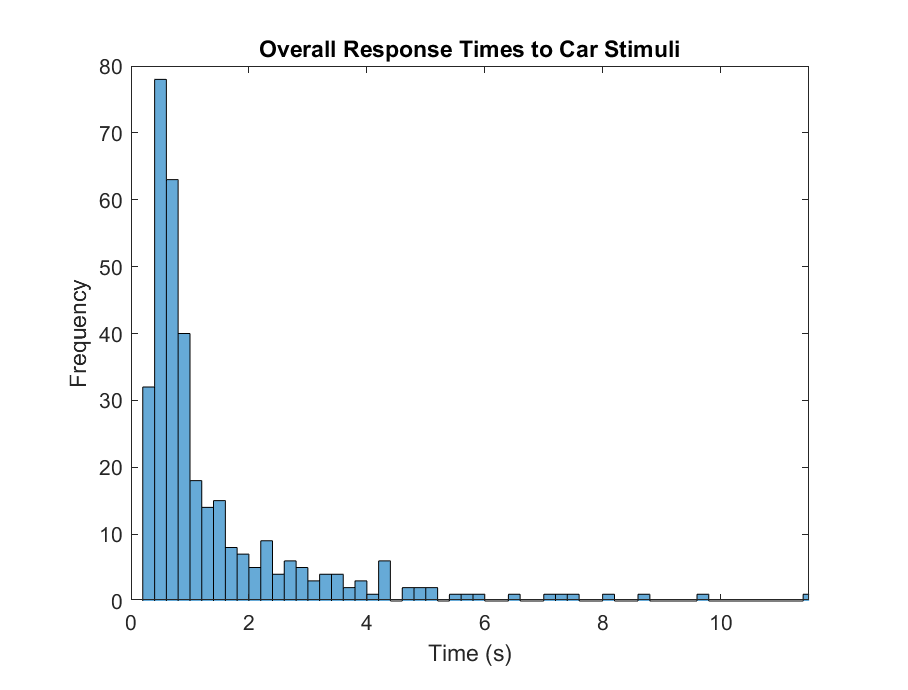
\includegraphics[width=0.37\paperwidth]{figures/CarReactionTimes.eps}
    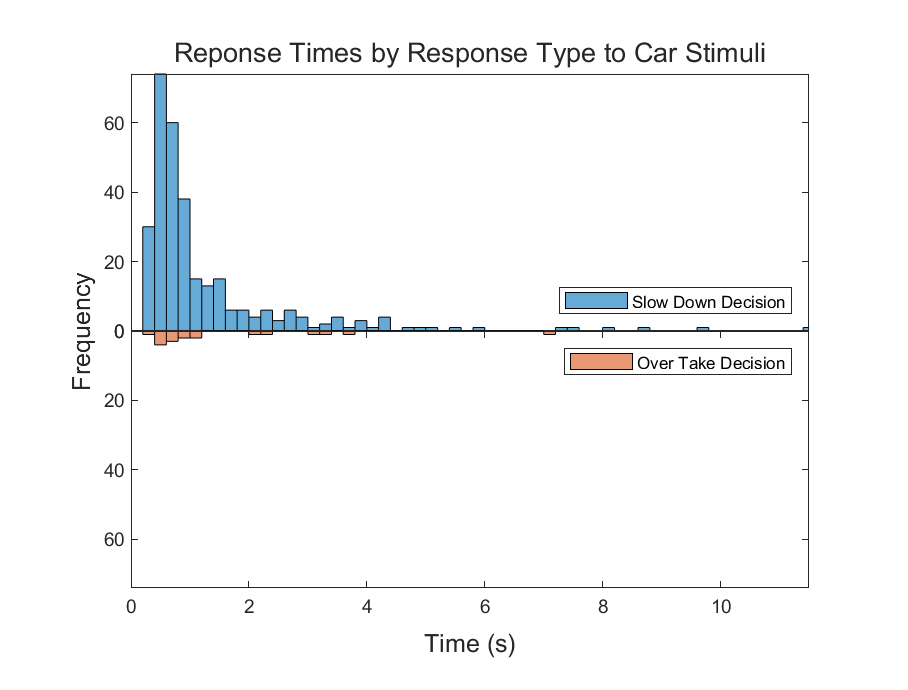
\includegraphics[width=0.37\paperwidth]{figures/CarReactionTimes2.eps}
    \caption{Non-Subject Specific Distribution of Response Times to the 'Car' Stimulus. a) Not Segregated by Response Type b) Segregated by Response Type}
    \label{fig:RT_C}
\end{figure}

As can be clearly seen in figure \ref{fig:RT_C} the number of 'incorrect' overtake responses to the 'Car' stimuli is negligible. Having confirmed that the reaction time distributions follows that of a typical decision task the next step was to examine the overarching question of this package of work. What factors influence the 2AFC decisions made during this task.

Those response time plots were then disaggregated by subject, summarised and tabulated in table \ref{tab:RSLT_responseSummary} below. Plots of the reaction time distributions for each subject can be found in appendix \ref{appendix:ExtraResults0_2}.
% Summary Reaction Time Results
\begin{table}[H]
    \begin{center}
        \caption{Tabulated Values of Response Time for Each Subject by Subject Type}
        \label{tab:RSLT_responseSummary}
        \begin{tabular}{cccccc}
        \hline
        \multirow{2}{*}{Subject} & \multirow{2}{*}{Overall Mean (s)} & \multicolumn{2}{c}{Cyclist Mean (s)} & \multicolumn{2}{c}{Car Mean (s)}  \\ \cline{3-6} 
                                &           & Overtaking    & Slowing Down  & Overtaking & Slowing Down \\ \hline
        a                       &   2.92    & 4.70          & 2.76          & 3.40      &   1.44        \\
        b                       &   1.90    & 4.52          & 2.30          & 3.13      &   0.85        \\
        c                       &   2.87    & 5.29          & 2.78          & 0.51      &   1.87        \\
        d                       &   2.16    & 3.31          & 1.56          & 0.77      &   1.53        \\
        e                       &   2.14    & 3.42          & 2.12          & 2.28      &   0.90        \\
        f                       &   2.17    & 3.97          & 2.72          & 0.52      &   1.13        \\ \hline
        \end{tabular}
    \end{center}
\end{table}

Those tabulated values can then be presented in a graph to examine the average response time by subject for each decision type and response, see figure \ref{fig:RT_SubjectMean}.
\begin{figure}[H]
    \centering
    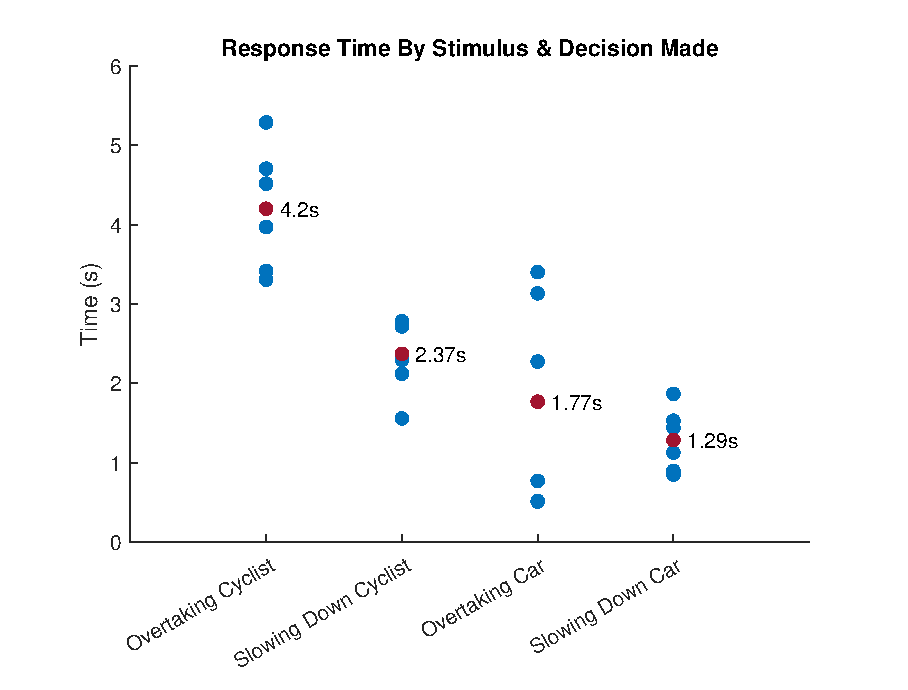
\includegraphics[width=0.6\linewidth]{figures/ReactionTimeMean.eps}
    \caption{Subject Mean Response Time by Stimulus \& Decision Made, Including the Aggregate Mean Values}
    \label{fig:RT_SubjectMean}
\end{figure}

This method can be extrapolated to examine the number of each decisions made which can be found in table \ref{tab:RSLT_nDecisions}. Due to the task having a underlying pseudo-randomised poisson sampling rate, this cannot be determined ahead of time.
\begin{table}[H]
    \begin{center}
        \caption{Tabulated Values of Number of Decisions Made by the Subjects}
        \label{tab:RSLT_nDecisions}
        \begin{tabular}{ccccc}
        \hline
        Subject &   Cyclist Decisions   & Car Decisions & Missed Decisions & Total Decisions \\ \hline
        a       &   57  & 53    & 7     & 117   \\
        b       &   55  & 47    & 5     & 107   \\
        c       &   62  & 60    & 7     & 129   \\
        d       &   40  & 46    & 7     & 93    \\
        e       &   64  & 65    & 2     & 131   \\
        f       &   50  & 54    & 10    & 114   \\ \hline
        \end{tabular}
    \end{center}
\end{table}

\section{Factors Influencing Driver Choice}
The factors examined in this analysis were those that the task was constructed around namely the 'View Distance' parameter, its corresponding 'Gap Distance' and the 'Cyclist Appearance Distance'.

\subsection{View \& Gap Distance}
Part of the task validation required the examination of the factors which were hypothesised to have an influence on the choice made by subjects. One of these factors which had been built into the task was the 'Perceived Gap' distance, discussed in \ref{MET:perceivedGap}. A major discovery following the pilot trials was that the gap distance is functionally the same as the camera's view distance. This effect can be seen in figure \ref{fig:Gap_more_like_view} where the levels of the view distance factor overwhelmingly dominate the distribution of the parameter.
\begin{figure}[H]
    \centering
    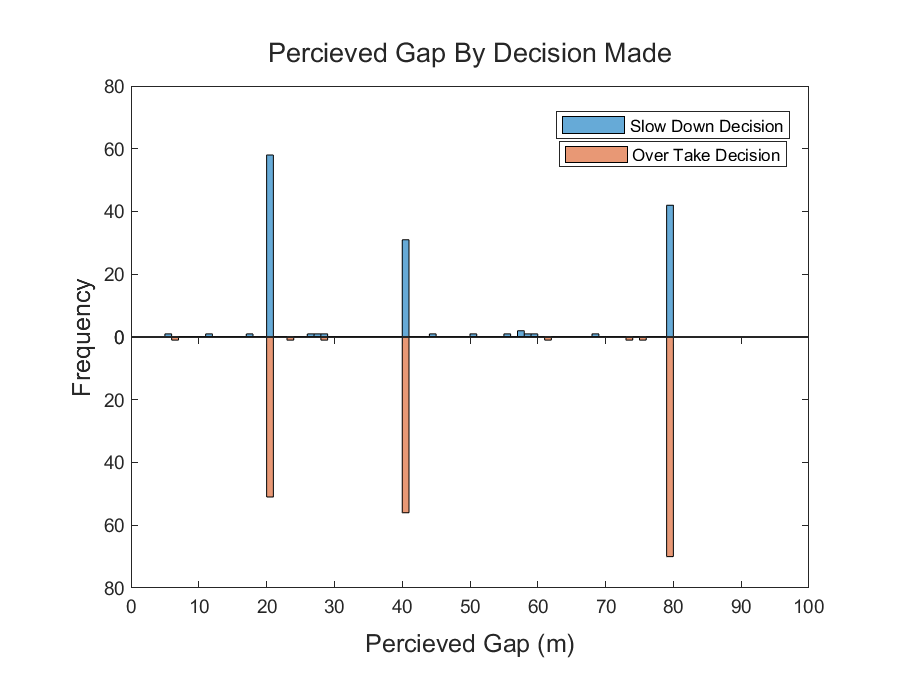
\includegraphics[width=0.6\linewidth]{figures/gap_hist.eps}
    \caption{Histogram Showing The 'Perceived Gap' at All Decision Points. Note: The Overwhelming Effect of The View Distance Levels}
    \label{fig:Gap_more_like_view}
\end{figure}

It was hypothesised that the view distance would be an influencing factor in the decisions made by subjects. To examine this hypothesis the decisions made were plotted as in figure \ref{fig:Proportion by View Dist}. It can be seen that the proportion of overtakes is lower in the smallest $20m$ view distance, but there is not as clear a trend at the $40m$ \& $80m$ levels.
% Proportion by 
\begin{figure}[H]
    \centering
    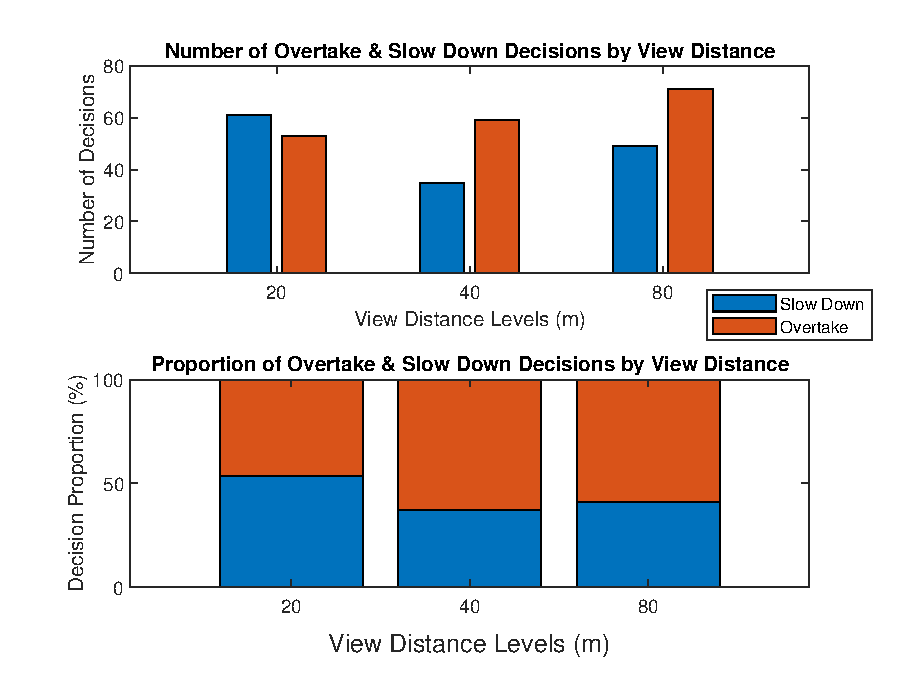
\includegraphics[width=0.6\linewidth]{figures/Proportions_by_viewdist.eps}
    \caption{Bar Chart Showing Details of Decisions Made by View Distance a) Number of Each Decision Made by View Distance b) Proportion of Each Decision Made by View Distance}
    \label{fig:Proportion by View Dist}
\end{figure}

\subsection{Cyclist Appearance Distance}
Another factor of interest was the distance from the camera where the cyclist stimulus first appeared. The distributions of this factor were plotted in figure \ref{fig:CyclistPositionDist}. In a) the $40m$ \& $60m$ levels can be seen to closely correlate with each other with a large spike at approx. $2s$ response time with a secondary spike at approx. $7s$. The $20m$ level has a flatter distribution and a longer tail. In b)i) we see the slow down decision also exhibits this early spike behaviour in the higher view distances.
\begin{figure}[H]
    \centering
    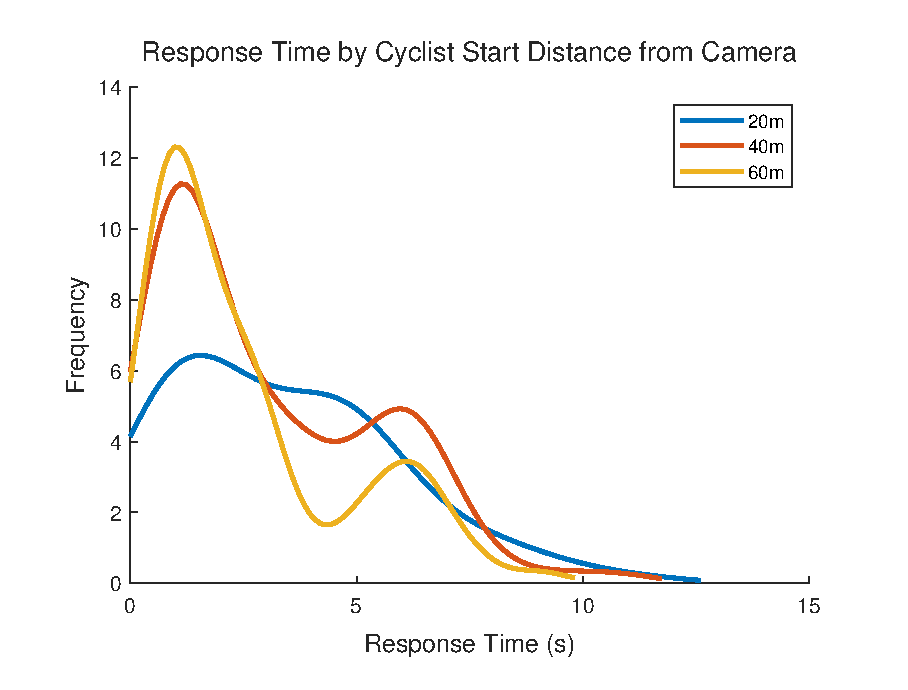
\includegraphics[width=0.37\paperwidth]{figures/CycleDist_overall.eps}
    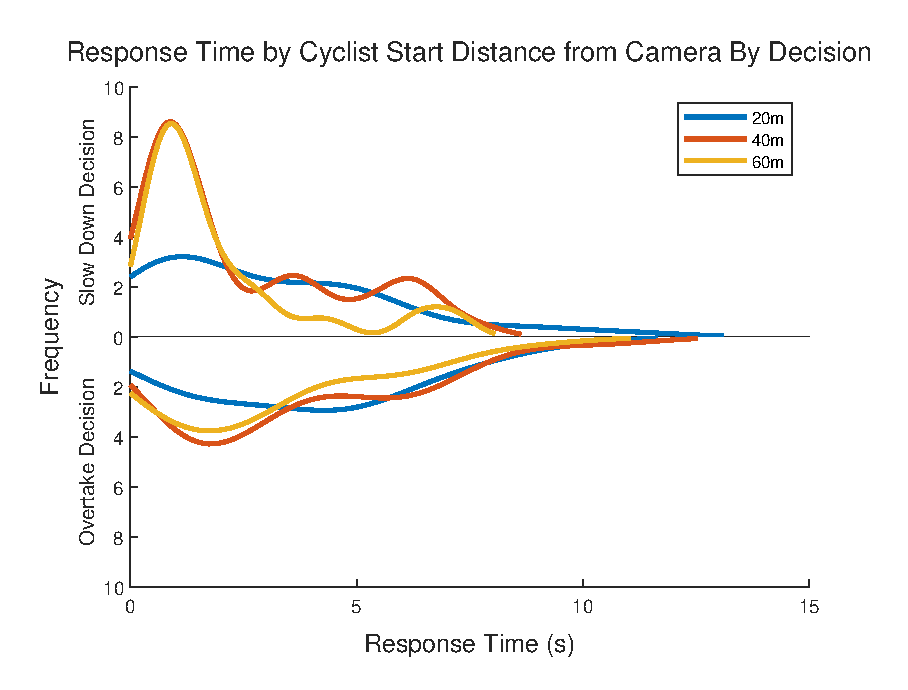
\includegraphics[width=0.37\paperwidth]{figures/CycleDist_byDecision.eps}
    \caption{Response Time Distributions by a) Cyclist Start Distance b) And Further Broken Down by i) Slow Down Decision ii) Overtake Decision}
    \label{fig:CyclistPositionDist}
\end{figure}



\section{Interpersonal Differences}
Plotting the proportion of each choice made by subject reveals a stark underlying inter-subject difference. It can be clearly seen in figure \ref{fig:Underlying_biases} that the dominant factor in which choice is made is the biases each subject has to those choices.
% Proportion by subject
\begin{figure}[H]
    \centering
    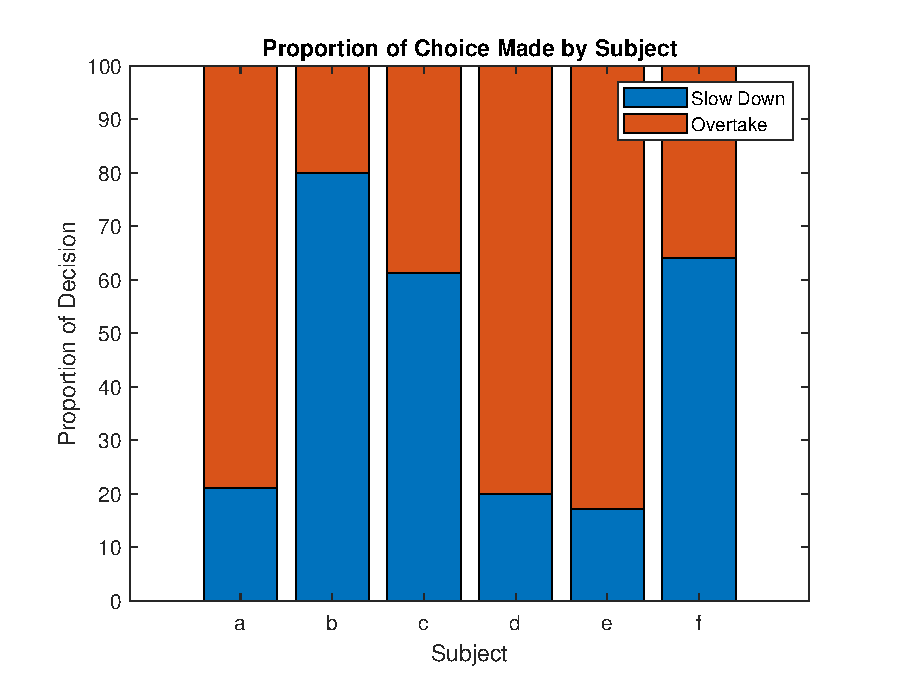
\includegraphics[width=0.75\linewidth]{figures/Proportions_by_sub.eps}
    \caption{Bar Chart Showing Proportion of Each Choice Made By Each Subject}
    \label{fig:Underlying_biases}
\end{figure}

\section{Subject Speed Setting}
\begin{figure}[H]
    \centering
    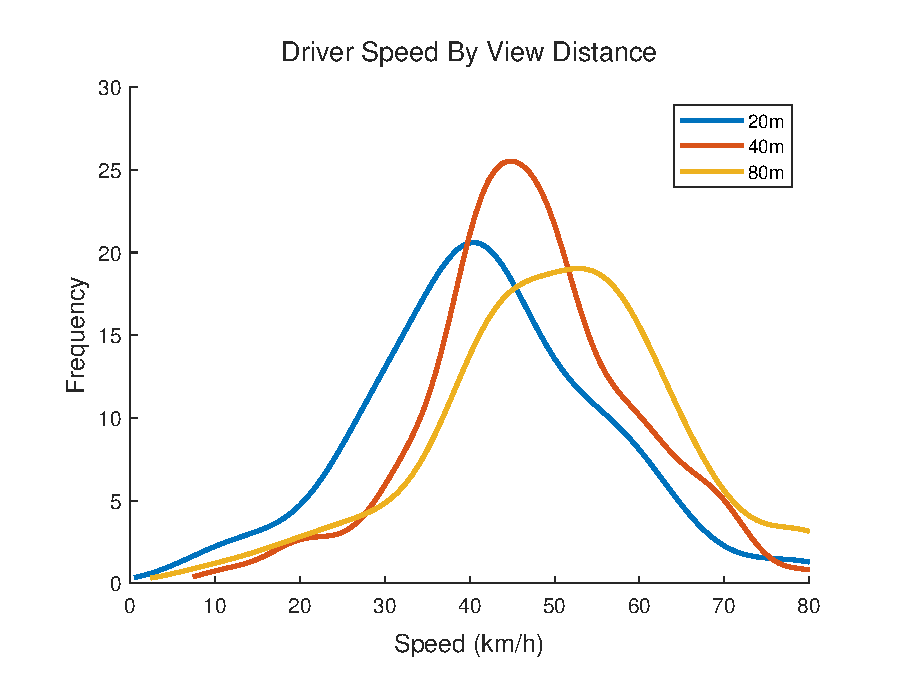
\includegraphics[width=0.75\linewidth]{figures/Speed_Setting_By_View_Dist.eps}
    \caption{Distribution of Speed Disaggregated by View Distance}
    \label{fig:Speed_Setting}
\end{figure}

These distributions were then compared using a one-way ANOVA and a statistical difference was found between the groups (p=0.000, $\alpha$=0.05). This suggests that subjects set their speed based on the view distance, a result that was expected. A pairwise comparison using Tukey's method was conducted and the results shown in table \ref{tab:RSLT_Pairwise}. As can be seen in the table, there were significant differences identified between the $20m$ setting and both the $40m$ \& $80m$. However, no significant difference was identified between the latter two groups.

\begin{table}[H]
    \begin{center}
        \caption{Speed - View Distance Pairwise Comparison Table}
        \label{tab:RSLT_Pairwise}
        \begin{tabular}{c|c|c}
        \hline
        Group 1 &   Group 2 &   p-Value     \\ \hline
        20m       &   40m   &   0.018       \\
        20m       &   80m   &   0.000       \\
        40m       &   80m   &   0.203       \\ \hline
        \end{tabular}
    \end{center}
\end{table}

\section{The Effect of Driver Speed on Choice}
The speed of the driver is a variable set by the subject of the task. In figure \ref{fig:Speed_By_Decision} a) we can see the differences between the speed distributions at the decision time. The distributions have a similar shape and mode, however, the overtake distribution contains a secondary 'hump' at approx. $55 km/h$. This is further detailed by the view distance at decision time. In this plot it can be seen that the higher view distances skew the mean of the distributions towards the maximum allowed speed of approx. $80 km/h$. This suggest that the effect of view distance speed-setting dominates this result.

\begin{figure}[H]
    \centering
    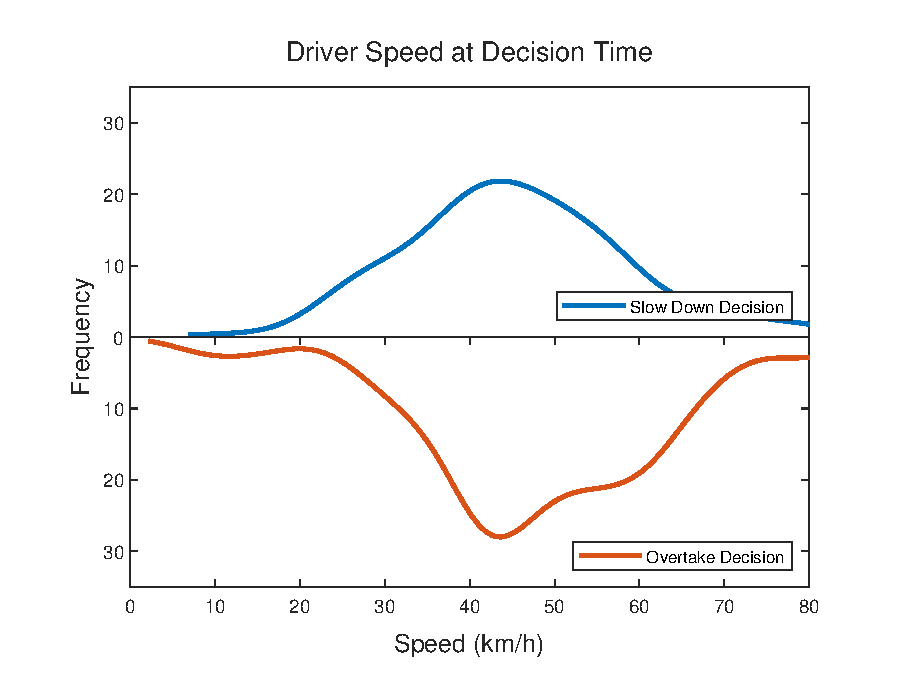
\includegraphics[width=0.37\paperwidth]{figures/Speed_Decision_Response.eps}\hfill
    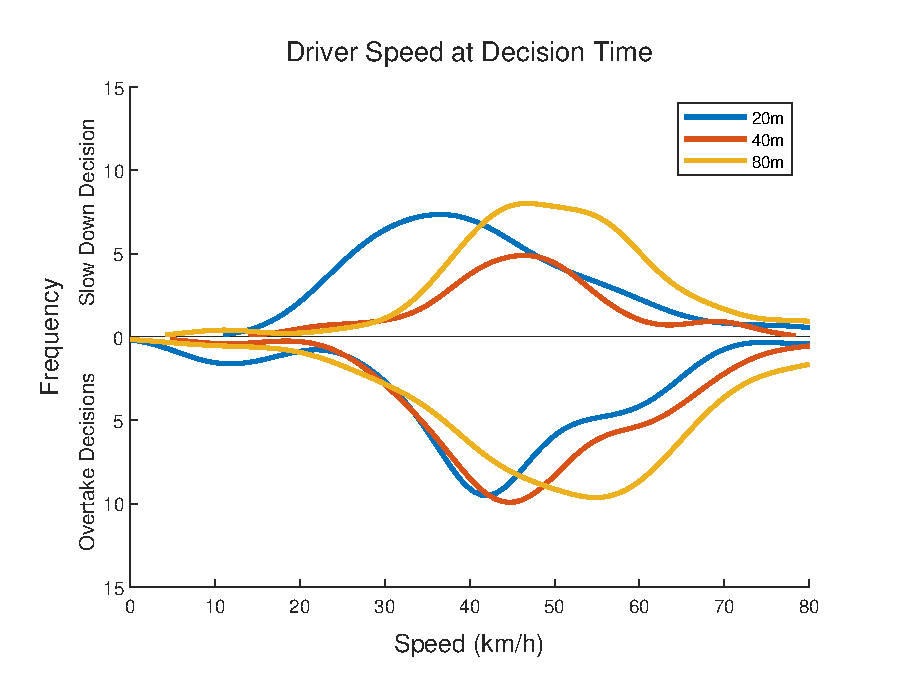
\includegraphics[width=0.37\paperwidth]{figures/Speed_Decision_Response_by_view_Dist.eps}
    \caption{Plots Showing the Driver Speed Immediately Prior to a Decision a) Aggregated Data Showing All Decisions b) Disaggregated By View Distance at Decision Time}
    \label{fig:Speed_By_Decision}
\end{figure}